% !TEX root = main.tex
\documentclass[10pt, a4paper]{article}

% ── Packages ──────────────────────────────────────────────────────────────────
\usepackage[
  top=0.35in, bottom=0.35in,
  left=0.45in, right=0.45in
]{geometry}
\usepackage[dvipsnames]{xcolor}
\usepackage{hyperref}
\usepackage{graphicx}
\usepackage{titlesec}
\usepackage{enumitem}
\usepackage{array}
\usepackage{tabularx}
\usepackage{parskip}

% ── Hyperlink styling ─────────────────────────────────────────────────────────
\hypersetup{
  colorlinks=true,
  urlcolor=black,
  linkcolor=black
}

\pagestyle{empty}

% Section formatting
\titleformat{\section}
  {\normalsize\bfseries}
  {}{0em}{\MakeUppercase}
  [\vspace{-6pt}\rule{\linewidth}{0.5pt}]

\titlespacing{\section}{0pt}{6pt}{2pt}

\setlist[itemize]{noitemsep, topsep=0pt, partopsep=0pt, parsep=0pt, leftmargin=1.2em, itemsep=0pt}

\setlength{\parindent}{0pt}
\setlength{\parskip}{0pt}

% Set base font size slightly larger than 10pt default
\fontsize{10.5}{13.5}\selectfont

% ══════════════════════════════════════════════════════════════════════════════
\begin{document}

% ── HEADER ────────────────────────────────────────────────────────────────────
\noindent
\begin{minipage}[c]{0.48\textwidth}
  \raggedright
  {\fontsize{24}{28}\selectfont \textbf{YOUR NAME}}\par
  \vspace{5pt}
  {\large\itshape\color{gray} Mobile Application Developer}\par
\end{minipage}%
\hfill
\begin{minipage}[c]{0.36\textwidth}
  \raggedleft
  \begin{minipage}[c]{0.68\linewidth}
    \raggedleft
    {\small\itshape\color{gray}
      \href{mailto:your.email@example.com}{your.email@example.com}\\[3pt]
      +91\,00000\,85302\\[3pt]
      \href{https://linkedin.com/in/your-linkedin}{linkedin.com/in/your-linkedin}\\[3pt]
      \href{https://github.com/your-github}{github.com/your-github}\\
    }
  \end{minipage}%
  \hspace{0.1pt}
\begin{minipage}[c]{0.26\linewidth}
    \raggedleft
    \fboxsep=2pt\fboxrule=0.5pt
    \fbox{%
      \IfFileExists{../../assets/profile-photo.jpg}{%
        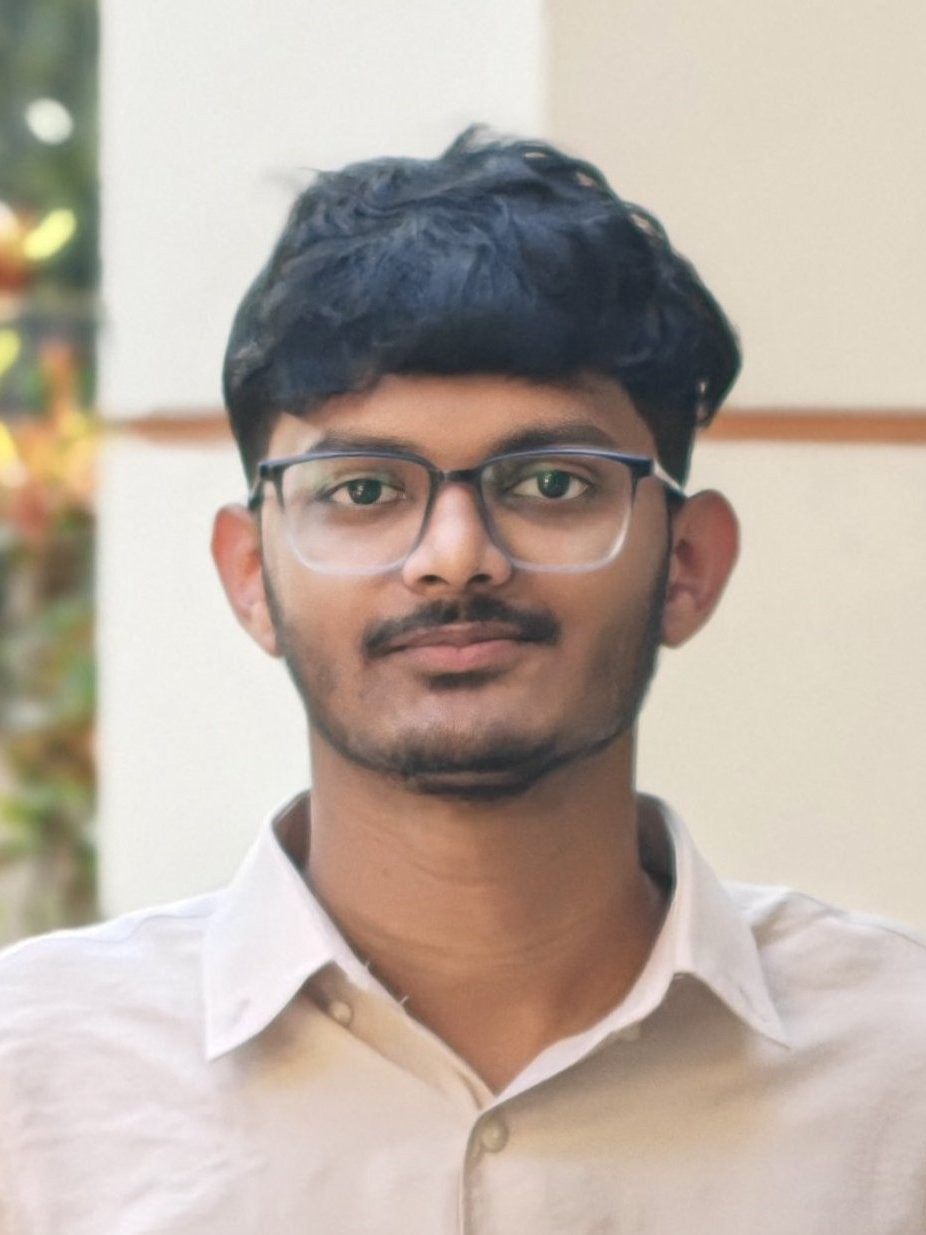
\includegraphics[height=0.75in,keepaspectratio]{../../assets/profile-photo.jpg}}{%
      \IfFileExists{../../assets/profile-photo.png}{%
        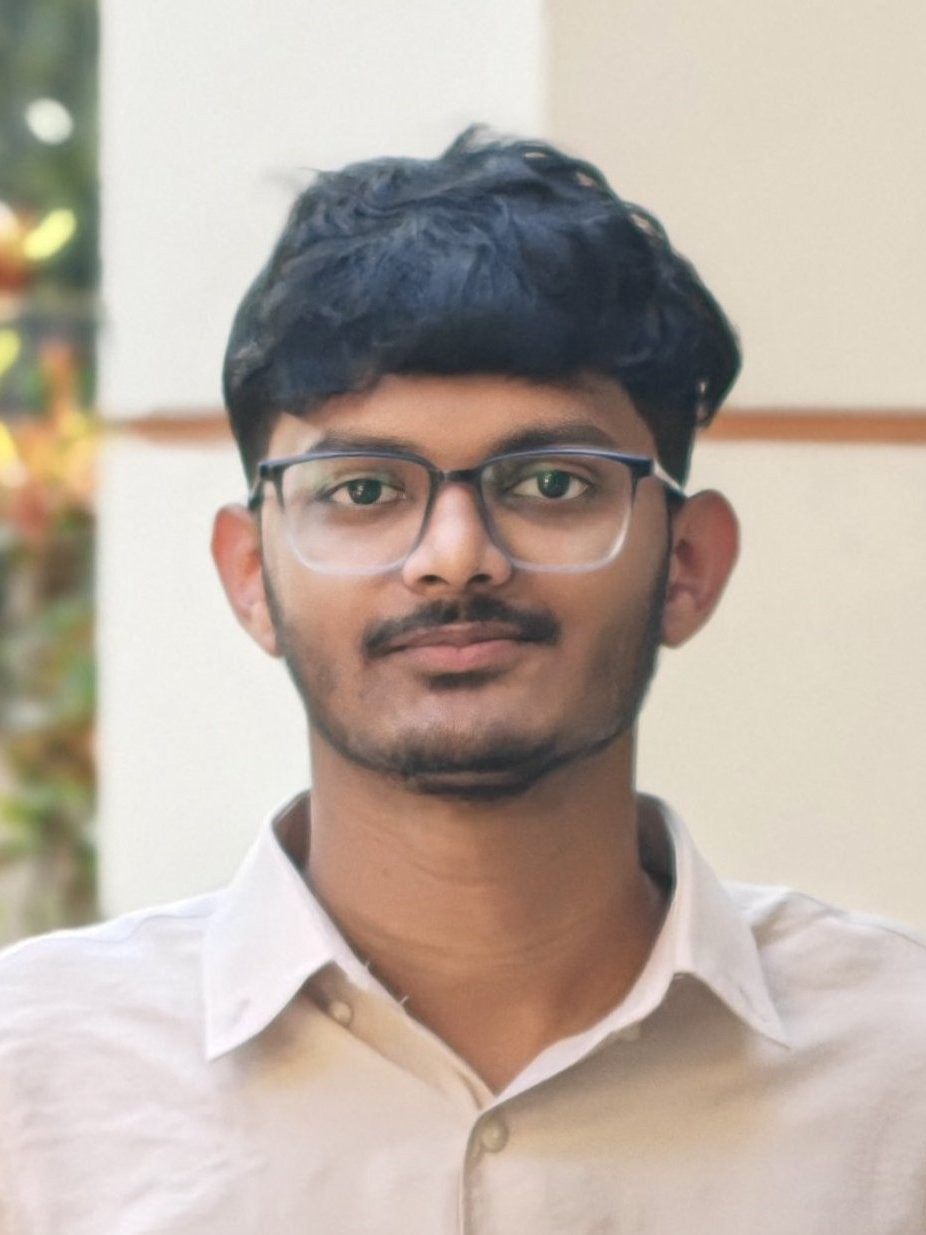
\includegraphics[height=0.75in,keepaspectratio]{../../assets/profile-photo.png}}{%
      \IfFileExists{../../assets/photo.jpg}{%
        \includegraphics[height=0.75in,keepaspectratio]{../../assets/photo.jpg}}{%
      \IfFileExists{../../assets/photo.png}{%
        \includegraphics[height=0.75in,keepaspectratio]{../../assets/photo.png}}{}}}}%
    }%
  \end{minipage}
\end{minipage}


% ── YOUR RESUME CONTENT GOES BELOW ───────────────────────────────────────────
\section*{Professional Summary}

Mobile Application Developer specializing in cross-platform app development and real-time systems. Proficient in Flutter and Firebase, with experience building responsive mobile interfaces, integrating device-level features, and delivering scalable user-focused applications.

%------------------------------------------------------------
% TECHNICAL SKILLS
%------------------------------------------------------------
\section*{Skills}

\renewcommand{\arraystretch}{1.05}
\begin{tabular}{@{} >{\bfseries}p{3.8cm} p{13cm} @{}}
Languages           & Dart, JavaScript, TypeScript, Python, Java, C \\
Mobile Development  & Flutter, Firebase, Android SDK ADB, React Native \\
Frameworks          & Node.js, Next.js, React.js, Express.js, Tauri, Wails \\
Backend \& APIs     & Flask, Django, REST APIs, Supabase, PHP \\
Databases           & MongoDB, MySQL \\
Developer Tools     & Git, GitHub, Docker, Postman, Android Studio \\
Operating Systems   & Linux , Windows \\
\end{tabular}

%------------------------------------------------------------
% PROJECTS
%------------------------------------------------------------
\section*{Projects}

\textbf{IRRIGO -- Smart Irrigation Platform} \hfill \textit{Flutter, Firebase, Next.js, Flask \quad Oct 2024}
\begin{itemize}
\item Developed a cross-platform mobile application for real-time farm monitoring and irrigation control.
\item Improved water usage efficiency by \textasciitilde{}20\% through data-driven insights accessible via mobile dashboard.
\item Integrated real-time weather and satellite data for responsive mobile-based decision support.
\end{itemize}

\vspace{3pt}

\textbf{DroidOps -- Android Device Management GUI} \hfill \textit{Tauri, React, TypeScript \quad Dec 2025} \quad \href{https://github.com/your-github/droidops}{GitHub}
\begin{itemize}
\item Engineered a device management interface leveraging Android Debug Bridge ADB for multi-device interaction.
\item Optimized execution workflows, improving command responsiveness and device interaction efficiency by \textasciitilde{}40\%.
\item Enabled real-time monitoring and debugging of Android devices through streamlined UI workflows.
\end{itemize}

\vspace{3pt}

\textbf{AI-Based Smart Traffic System Using Computer Vision} \hfill \textit{Python, YOLO, Flask \quad Jan 2025}
\begin{itemize}
\item Developed a real-time traffic monitoring system with mobile-responsive dashboard for live insights.
\item Achieved 92--94\% detection accuracy with optimized inference latency less than 200ms per frame.
\item Designed system architecture adaptable for edge/mobile deployment in smart city environments.
\end{itemize}

\vspace{3pt}

\textbf{Certificate Generator and Verification System} \hfill \textit{Node.js, Firebase \quad Dec 2024} \quad \href{https://github.com/your-github/advanced-certificate-generator}{GitHub}
\begin{itemize}
\item Built a QR-based verification system enabling instant certificate validation on mobile devices.
\item Automated bulk certificate generation for 1,000+ records per batch, reducing manual effort by \textasciitilde{}85\%.
\item Developed responsive interfaces ensuring seamless mobile and web accessibility.
\end{itemize}

%------------------------------------------------------------
% EDUCATION
%------------------------------------------------------------
\section*{Education}

\textbf{B.Tech in Computer Science and Engineering} \hfill \textbf{2022 -- 2026}\\
Mar Baselios Christian College of Engineering and Technology, Kuttikkanam \hfill APJ Abdul Kalam Technological University

%------------------------------------------------------------
% CERTIFICATIONS
%------------------------------------------------------------
\section*{Certifications}

\renewcommand{\arraystretch}{1.1}
\begin{tabular}{@{} p{7.8cm} p{6.5cm} p{2.5cm} @{}}
\textbf{Certificate}                  & \textbf{Issuer}              & \textbf{Year} \\[1pt]
Programming with Python               & Python Institute OpenEDG   & 2024 \\
Python for Data Science               & NPTEL -- IIT Madras          & 2024 \\
JavaScript Foundations Professional   & Mozilla                      & Jul 2025 \\
Amazon API Gateway for Serverless     & AWS Training                 & Jun 2025 \\
Ubuntu Linux Professional Certificate & Canonical                    & Nov 2025 \\
\end{tabular}

%------------------------------------------------------------
% ACHIEVEMENTS
%------------------------------------------------------------
\section*{Achievements}

\begin{tabular}{@{} p{9.5cm} p{8cm} @{}}
Galactic Problem Solver              & NASA Space Apps Challenge 2024 \\
Global Connection Recognition        & NASA Space Apps Challenge 2025 \\
Global Nominee                       & NASA Space Apps Challenge 2025 \\
\end{tabular}

%------------------------------------------------------------
% INTERESTS & LANGUAGES
%------------------------------------------------------------
\section*{Additional Information}

\begin{tabular}{@{} >{\bfseries}p{3.8cm} p{13cm} @{}}
Areas of Interest & Mobile Application Development, Flutter, Android Development, Cross-Platform Development, Firebase, UI Development, REST API Integration, Mobile UI/UX \\
Languages         & English Professional, Malayalam Native \\
\end{tabular}

\end{document}
